\newpage
\section{Superconducting Qubits}

\subsection{Conductors and Superconductors}

\subsubsection{Simple Metals}
The tight-binding model in Lab 6 is a good starting point to understand conductors, in particular, metals. 

Fermi energy $E_F$.

the density of states
\begin{align*}
    \nu(E)\propto  E^{\frac{1}{2}}
\end{align*}

As a result, the energy dissipation in metals are characterized by a finite resistivity
\begin{align*}
    \rho=\frac{m}{ne^2 \tau }
\end{align*}
where $\tau$ is the average collision time. 

\subsubsection{Superconductivity}
From microscopic point of view, the Fermi sea in a metal is unstable under attractive electron-electron interaction mediated by phonons, or lattice vibrations. As a result, electrons with opposite momentum $\vec{k}$ and spin $\sigma$ pair in $k$-space are locked into Cooper pairs and form a coherent state

\begin{figure}[H]
    \centering
    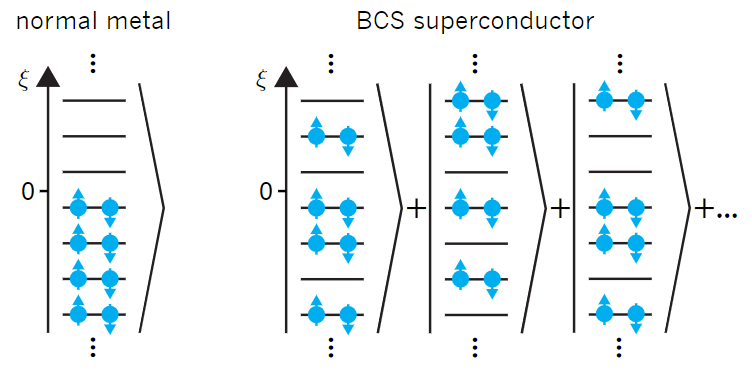
\includegraphics[width=0.309\textwidth]{QI9/electrons form a coherent state}
    \caption{Electrons form a coherent state}
\end{figure}

The electron pairs can be broken to create a pair of (Bogoliubov) quasiparticles. 

\begin{figure}[H]
    \centering
    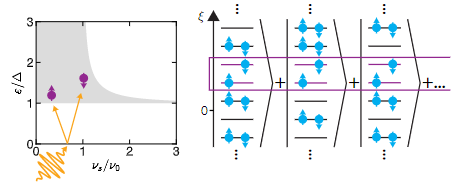
\includegraphics[width=0.309\textwidth]{QI9/create a pair of quasiparticles}
    \caption{create a pair of quasiparticles}
\end{figure}

Due to the attractive electron-electron interaction mediated by phonons, this process requires a minimum energy of $2\Delta$, where $\Delta$ is know as the superconducting gap. For aluminum, this gap is about 1 K. 

When temperature is sufficiently low ($k+B T \ll \Delta$), the system condenses into the coherent state, known as the Bardeen-Cooper-Schrieffer (BCS) state. 

Only unpaired quasiparticles can be scattered by impurities,
hence dissipating energy to the lattice. But their number is
exponentially suppressed at low temperatures
\begin{align*}
    n_{qp}\sim e^{-\Delta / (k_B T)}
\end{align*}
according to the Boltzmann distribution.

Therefore, a superconductor can be thought of as a macroscopic quantum state, characterized by the number $N_s$ of superconducting electron pairs.


\subsection{Tunneling Junctions and The Josephson Effect}

\subsubsection{Normal-State Tunneling Junction}

Consider a tunneling junction, where two normal-state metallic leads are separated by a thin oxide, or a tunnelling barrier. Due to quantum tunnelling electrons can penetrate through the barrier.
\begin{figure}[H]
    \centering
    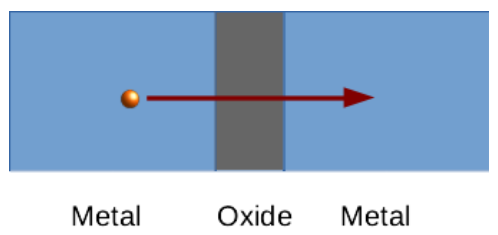
\includegraphics[width=0.309\textwidth]{QI9/Normal-State Tunneling Junction}
    \caption{Normal-State Tunneling Junction}
\end{figure}

\begin{figure}[H]
    \centering
    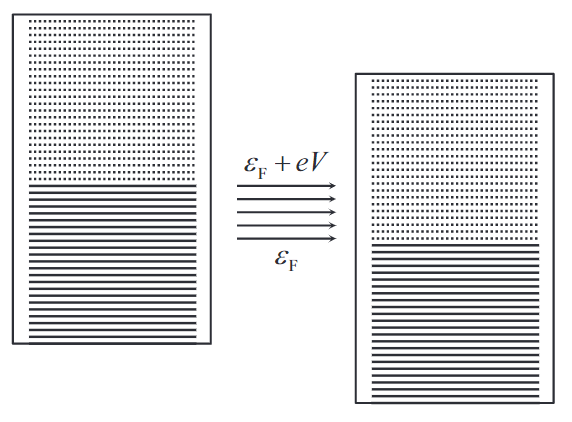
\includegraphics[width=0.309\textwidth]{QI9/two metals}
    \caption{two metals with insulator between}
\end{figure}

When the Fermi energies on the two sides are shifted by a small voltage bias $V$ (low compared to the barrier height), electrons in the resulting energy interval $e$V are able to tunnel from one side to the other without blocking due to the Pauli exclusion principle. 

As a result the tunnel current is linear in $V$ and the junction can be characterized as a simple resistor with resistance $R_N$ . One can show
\begin{align*}
    G_N=\frac{1}{R_N} \propto \frac{e^2}{h}(\nu_L \nu_R)t^2
\end{align*}
where $t$ is the energy gain from tunneling, and $\nu_{L,R}$ are the densities of states of the two leads.

\subsubsection{Superconducting Tunneling Junction}
When we cool the two metallic leads below their superconducting transition temperature, they become superconducting leads.

\begin{figure}[H]
    \centering
    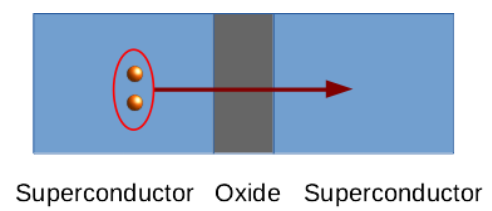
\includegraphics[width=0.309\textwidth]{QI9/Superconducting Tunneling Junction}
    \caption{Superconducting Tunneling Junction}
\end{figure}
Now, dissipation is negligible, and the tunneling resistance is replaced by a non-linear inductor. The physical picture is that quantum wave functions on the two sides overlap with each other in the barrier. Therefore, Cooper pairs can still flow, leading to what is known as the supercurrent (though, on a weaker scale of the order of 10 A/cm${}^2$), hrough the tunneling barrier where the superconducting gap is strongly suppressed (hence, a weak link).

This is a striking manifestation of the quantum nature of superconductivity, known as the Josephson effect. It leads to the only known non-linear non-dissipative circuit element, \textbf{the Josephson junction (Josephson 结)}.

\subsubsection{The Josephson Effect}

In the limit of low temperatures $k_B T\ll 2\Delta$ and low frequencies $\hbar \omega \ll 2\Delta$, we can model electrons in each lead by a single quantum state $\ket{N}$, labeled by the number of electron pairs. For the two leads connected by a tunnel junction, there is a large family of degenerate ground states $\ket{N_L, N_R}$, labeled by the number of Cooper pairs in the two leads.

Note $N_L + N_R$ is a constant due to charge conservation. We can, alternatively, use $m = (N_R - N_L)/2$ to represent the family of states as
\begin{align*}
    \ket{m}\equiv \ket{N_L, N_R}
\end{align*}


The tunneling of a Cooper pair leads to the change of $m$ by
1, like a particle hopping to an adjacent site on a lattice.

\begin{figure}[H]
    \centering
    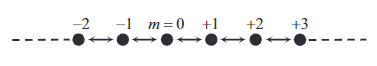
\includegraphics[width=0.309\textwidth]{QI9/the family of states}
    \caption{the family of states}
\end{figure}

Therefore, we consider the phenomenological Hamiltonian
\begin{align*}
    \hat{H}_T=-\frac{1}{2}E_J\sum(\ket{m}\bra{m+1}+\ket{m+1}\bra{m})
\end{align*}
where $E_J$ is called the Josephson coupling energy, which is
related to the normal-state conductance $G_N$ by the Ambegaokar-Baratoff relation
\begin{align*}
    E_J=\frac{\Delta}{2}\frac{h}{(2e)^2}G_N
\end{align*}

We will find a linear superposition of the degenerate states that diagonalizes $\hat{H}_T$ (i.e., degenerate perturbation) and finding energy eigenvalues, which is first order in $E_J$. 

The eigenstates are
\begin{align*}
    \ket{\varphi }=\sum_{m=-\infty}^{+\infty}e^{im\varphi}\ket{m}
\end{align*}
where $\varphi$ is like wave vector ``$k$'', if we think $m$ as a site. 

In the $\varphi$ representation, a wave function is given by
\begin{align*}
    \psi(\varphi)=\braket{\varphi|\psi}=\sum_{m=-\infty}^{+\infty}e^{-im\varphi}\braket{m|\psi}
\end{align*}

In an analogy to free electrons, the ``momentum'' operator is $\hbar \varphi$, and the ``position'' operator would be
\begin{align*}
    \hat{n}\equiv\sum_m\ket{m}m\bra{m}
\end{align*}

Hence,
\begin{align*}
    \bra{\varphi}(\hat{n}\ket{\psi})&=\sum_{m=-\infty}^{+\infty}e^{-im\varphi}\bra{m}\left( \sum_{m'}\ket{m'}m'\braket{m'|\psi} \right)\\
    &=\sum_{m=-\infty}^{+\infty}e^{-im\varphi}m\braket{m|\psi}\\
    &=i\frac{d}{d\varphi}\sum_{m=-\infty}^{+\infty}e^{-im\varphi}\braket{m|\psi}\\
    &=i\frac{d}{d\varphi}\psi(\varphi)
\end{align*}

Therefore, we find
\begin{align*}
    \hat{n}\equiv i\frac{d}{d\varphi}
\end{align*}

As we work out in Lab 6 for the tight-binding model,
\begin{align*}
    H_T \ket{\varphi}= E(\varphi)\ket{\varphi}=-E_J\cos\varphi\ket{\varphi}
\end{align*}

The ``group velocity'' would, then, be
\begin{align*}
    v_g(\varphi)=\frac{1}{\hbar}\frac{\partial}{\partial \varphi}(-E_J\cos\varphi)=\frac{E_J}{\hbar}\sin\varphi
\end{align*}

So the net current flowing is given by the \textbf{dc Josephson relation}
\begin{align*}
    I=(2e)v_g(\varphi)=I_c\sin \varphi
\end{align*}
where $I_c=\frac{2e}{h}E_J$. 

The maximum possible coherent (dissipationless) current $I_c$ occurs at $\varphi=\frac{\pi}{2}$ and is called the \textbf{critical current}.

\begin{figure}[H]
    \centering
    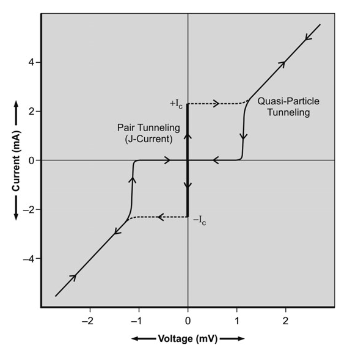
\includegraphics[width=0.309\textwidth]{QI9/critical current}
    \caption{critical current}
\end{figure}

If more current than this is forced through the junction, the low-energy effective model is no longer applicable. There is a finite resistance, and the voltage rises from zero to a high value above $2\Delta$. 

We consider the situation where an external electric field is applied and maintained in such a way that there is a fixed voltage drop $V$ across the tunnel junction. This adds to the Hamiltonian a ``potential'' term $U=-(2e)V\hat{n}$. 

The time rate of change of the ``momentum'' $\hbar\varphi$ to the `force' $2eV$ would be (notice $F = dp/dt$)
\begin{align*}
    \hbar\frac{d\varphi}{dt}=-\frac{dU}{d\hat{n}}=2eV
\end{align*}
or
\begin{align*}
    V=\frac{\hbar}{2e}\frac{d\varphi}{dt}
\end{align*}
This is known as the \textbf{ac Josephson relation}. 

Putting the two Josephson relations together, we see that a Josephson junction behaves as an inductor with a nonlinear inductance ($V=L_J \frac{dI}{dt}$)
\begin{align*}
    L_J(\varphi)=\frac{\hbar}{2e}\frac{1}{I_c\cos\varphi}=\left( \frac{\hbar}{2e} \right)^2\frac{1}{E_J\cos\varphi}
\end{align*}
and an inductive (kinetic) energy
\begin{align*}
    E(\varphi)=-E_J\cos\varphi
\end{align*}
Note that $\frac{dE}{dI}=\frac{dE(\varphi)}{d\varphi} / \frac{dI(\varphi)}{d\varphi} =L_J I$

\subsubsection{Charging Energy}
The tunneling of a Cooper pair transfers charge $2e$ from one to the other side of the junction. Due to Coulomb interaction, the junction also has a capacitance $C_J$ .

The energy associated with the transfer of $\hat{n}$ pairs of electrons is
\begin{align*}
    U&=\frac{Q^2}{2C}=\frac{(2e)^2}{2C}\hat{n}^2=4E_C \hat{n}^2 \\
    E_C&=\frac{e^2}{2C}
\end{align*}
In the absence of the additional capacitance, we have, here, $C = C_J$ .

\subsection{Superconducting Qubits}

We have studied a single isolated Josephson junction which is able to coherently transfer Cooper pairs from one superconducting island to another. 

With Coulomb interaction, an artificial atom can be realized and used as a qubit.

\begin{figure}[H]
    \centering
    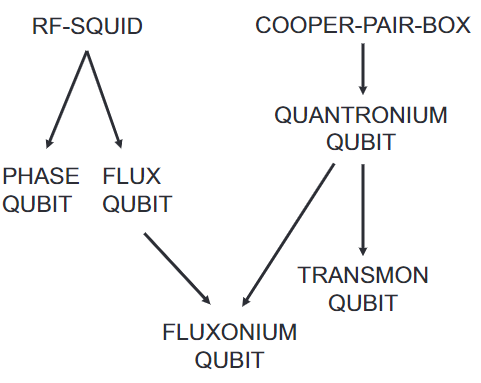
\includegraphics[width=0.309\textwidth]{Qi9/Superconducting Qubit Evolutionary Phylogeny}
    \caption{Superconducting Qubit Evolutionary Phylogeny}
\end{figure}


\subsubsection{The Cooper Pair Box}
A Cooper pair box qubit has a voltage source biasing the box through a coupling (`gate') capacitor $C_g$. 

\begin{figure}[H]
    \centering
    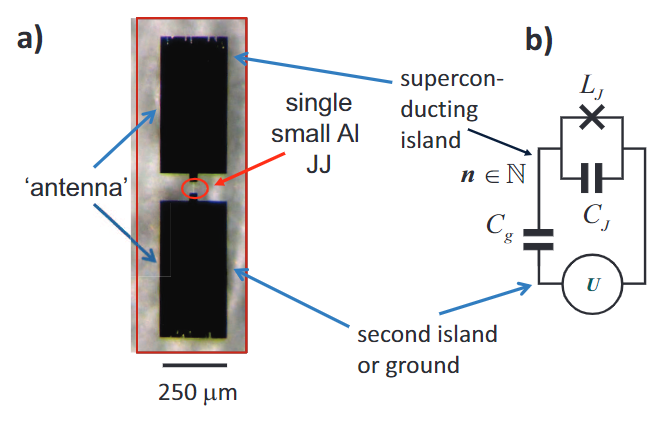
\includegraphics[width=0.309\textwidth]{QI9/The Cooper Pair Box}
    \caption{The Cooper Pair Box}
\end{figure}

The gate capacitor introduces a continuous offset $n_g = -C_g V /(2e)$, whose fluctuations can be overcome in the transmon qubit design.

Except for the $n_g$ term, the Hamiltonian becomes that of a quantum rotor in a gravitational field
\begin{align*}
    H=4E_C (\hat{n}-n_g)^2-E_J\cos\varphi
\end{align*}

\begin{figure}[!htb]
    \centering
    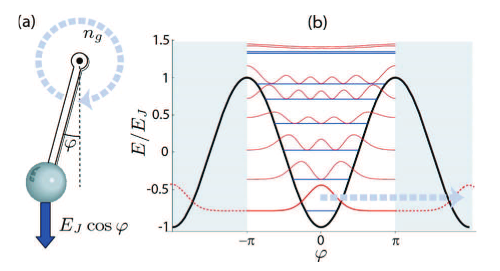
\includegraphics[width=0.42\textwidth]{Qi9/a quantum rotor in a gravitational field}
    \caption{a quantum rotor in a gravitational field}
\end{figure}

For small amplitude oscillations, the rotor is roughly a simple harmonic oscillator. This happens in the quantum case in the limit $E_J \gg E_C$ , where the zero-point fluctuations in the phase are small.

Up to an irrelevant constant in the energy (and ignoring the offset charge for the moment) we obtain
\begin{align*}
    H\approx 4E_C\hat{n}^2+\frac{1}{2}E_J\hat{\varphi}^2
\end{align*}
Notice $E_C = e^2/(2C)$, and $C = C_J + C_g$ is the total capacitance between the two superconducting islands.

% \begin{table}[H]
%     \centering
%     \caption{The comparison}
%     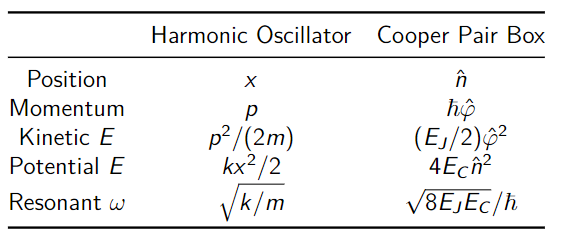
\includegraphics[width=0.409\textwidth]{QI9/The comparison}
% \end{table}

\begin{table}[H]
    \centering
    \caption{The comparison}
    \begin{tabular}[c]{ccc}\hline
        & Harmonic Oscillator & Cooper Pair Box\\ \hline
        Position & $x$ & $\hat{n}$ \\
        Momentum & $p$ & $\hbar\hat{\varphi}$ \\
        Kinetic $E$ & $\displaystyle \frac{p^2}{2m}$ & $\displaystyle \left( \frac{E_J}{2} \right)\hat{\varphi}^2$ \\
        Potential $E$ & $\displaystyle\frac{k x^2}{2}$ & $4E_C\hat{n}^2$ \\
        Resonant $\omega$ & $\displaystyle\sqrt{\frac{k}{m}}$ & $\displaystyle \frac{\sqrt{8E_J E_C}}{\hbar}$ \\ \hline
    \end{tabular}
\end{table}


The comparison leads to the resonant frequency of the CPB
\begin{align*}
    \Omega_J=\frac{1}{\hbar}\sqrt{8E_J E_C}
\end{align*}
The resonant frequency is also known as the Josephson plasma frequency
\begin{align*}
    \Omega_J&= \frac{1}{\sqrt{L_J(\varphi=0)C}}\\
    L_J&=\left( \frac{\hbar}{2e} \right)^2\frac{1}{E_J \cos\varphi}
\end{align*}
\begin{enumerate}\small
    \item The approximation we made replaces the Josephson junction by a linear inductance $L = L_J (\varphi = 0)$.
    \item The non-linear inductance of the junction will make the energy levels of the Cooper pair box anharmonic.
\end{enumerate}

\begin{figure}[!htb]
    \centering
    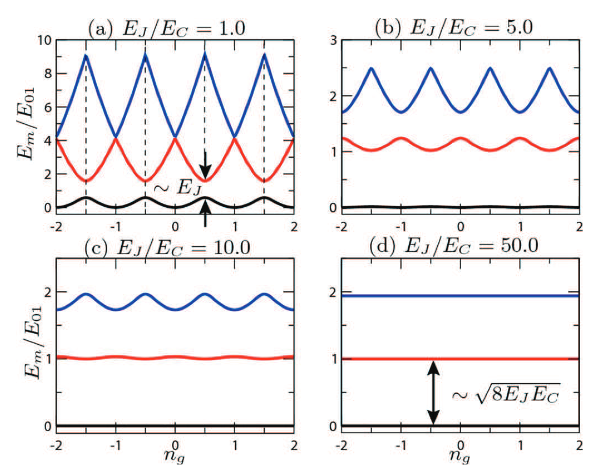
\includegraphics[width=0.429\textwidth]{QI9/Effect of increasing EJEC}
    \caption{Effects of increasing $E_J /E_C$}
\end{figure}
\begin{itemize}\small
    \item Good: Flatter energy levels, insensitive to charge fluctuations
    \item Bad: Decreasing anharmonicity
\end{itemize}

\subsubsection{Temperature}

The superconducting transition temperature $T_c$ of Al is about 1 K, which can be converted to 21 GHz.

So the operating temperature must satisfy $T\ll T_c$ . This is achieved by working inside a dilution refrigerator with base temperature about 30 mK.

The transition frequency of a qubit is usually a few GHz, which is much greater than $T$ , so thermal fluctuations are suppressed. Nevertheless, experiments have found a surprisingly large amount of nonequilibrium quasiparticles that lead to qubit energy relaxation $\ket{1}\rightarrow\ket{0}$. 